%\immediate\write18{tex calligraphy.dtx}
\immediate\write18{tex spath3.dtx}
\documentclass{article}
%\documentclass[convert={size=400},border=10]{standalone}
\usepackage{tikz}
\usetikzlibrary{decorations.pathreplacing,matrix,calligraphy}


\begin{document}

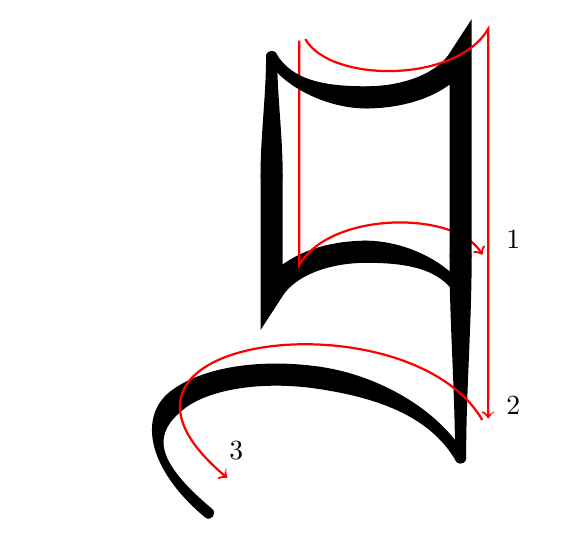
\begin{tikzpicture}[scale=2]
\calligraphy[
  copperplate,
  heavy line width=8pt,
  light line width=4pt,
  weight=heavy,
  annotate={draw,thick,red,->,shorten >=1ex,shorten <=1ex},
  annotation shift={(1em,1em)},
  annotation node style={1}{fill=white,fill opacity=.5,circle,text     opacity=1,anchor=south west},
  annotation node style={2}{fill=white,fill opacity=.5,circle,text     opacity=1,anchor=south west},
  annotation node style={3}{fill=white,fill opacity=.5,circle,text     opacity=1,anchor=south},
]
   (-.5,1.2) -- (-.5,-.3) .. controls +(60:.4) and +(120:.4) .. (.7,-.3)
   (-.5,1.2) .. controls +(-60:.4) and +(-120:.4) .. (.7,1.2) -- (.7,-1.35) +(0,0) .. controls +(120:1) and +(140:1.5) .. (-.9,-1.7)
;
\end{tikzpicture}
\end{document}

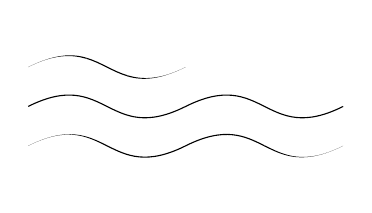
\begin{tikzpicture}
\pen (-20:.15) -- (20:.15);
\calligraphy[copperplate] (0,0) .. controls +(1,.5) and +(-1,-.5) .. (2,0);
\draw[yshift=-.5cm] (0,0) .. controls +(1,.5) and +(-1,-.5) .. (2,0) .. controls +(1,.5) and +(-1,-.5) .. (4,0);
\calligraphy[yshift=-1cm,copperplate] (0,0) .. controls +(1,.5) and +(-1,-.5) .. (2,0) .. controls +(1,.5) and +(-1,-.5) .. (4,0);
\end{tikzpicture}


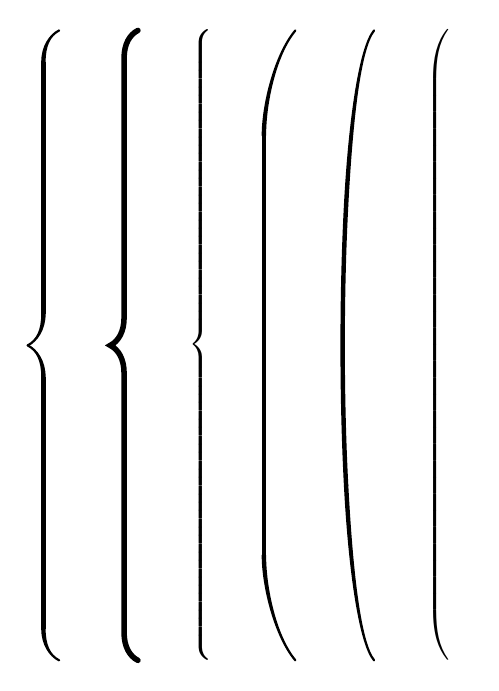
\begin{tikzpicture}
\draw[decorate,decoration={calligraphic brace,amplitude=4mm},ultra thick] (0,0) -- (0,8);
\draw[line width=2pt,decorate,decoration={brace,amplitude=10},line cap=round] (1,0) -- ++(0,8);
\node[anchor=south west,minimum height=8cm,outer sep=0pt,left delimiter=\{] (a) at (2,0) {};
\draw[decorate,decoration={calligraphic straight parenthesis,amplitude=4mm},ultra thick] (3,0) -- ++(0,8);
\draw[decorate,decoration={calligraphic curved parenthesis,amplitude=4mm},ultra thick] (4,0) -- ++(0,8);
\node[anchor=south west,minimum height=8cm,outer sep=0pt,left delimiter=(] (a) at (5,0) {};
\end{tikzpicture}

\begin{tikzpicture}[line width=2pt]
\pen (0,0) -- ++(.5,.5) ++(.5,.5);
\end{tikzpicture}


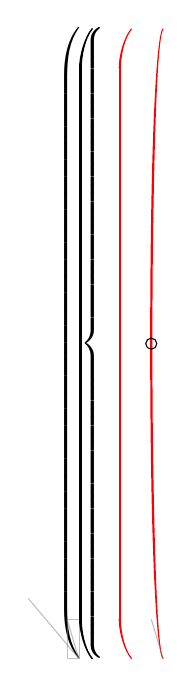
\begin{tikzpicture}
\node[anchor=south west,minimum height=8cm,outer sep=0pt,left delimiter=(] at (0,0) {};
\node[anchor=south west,minimum height=8cm,outer sep=0pt,left delimiter=\{] at (.3,0) {};
\draw[pen colour=red,decorate,decoration={calligraphic straight parenthesis,amplitude=1.5mm},thick] (.6,0) -- ++(0,8);
\draw[pen colour=red,decorate,decoration={calligraphic curved parenthesis,amplitude=1.5mm},thick] (1,0) -- ++(0,8);
\draw (.85,4) circle[radius=2pt];
\draw[gray,opacity=.5] (-.06,0) rectangle ++(-.15,.5);
\draw[gray,opacity=.5] (-.07,0) -- ++(130:1);
\draw[gray,opacity=.5] (-.07,0) -- ++(-.15,.5);
\calligraphy[copperplate,light,taper width=.5\pgflinewidth] (.1,0) .. controls +(130:.15) and +(0,-.15) .. ++(-.15,.5) -- ++(0,7) .. controls +(0,.15) and +(230:.15) .. ++(.15,.5);
\draw[gray,opacity=.5] (1,0) -- ++(-.15,.5);
\end{tikzpicture}

\begin{tikzpicture}
\pen[pen name=cplate] (0,0);
\calligraphy[pen name=cplate,red] (0,0) .. controls +(1,1) and +(-1,-1) .. ++(5,0);
\end{tikzpicture}

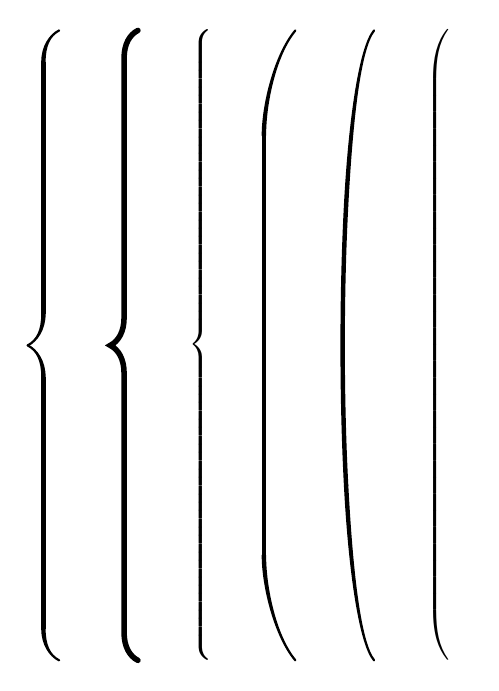
\begin{tikzpicture}
\draw[decorate,decoration={calligraphic brace,amplitude=4mm},ultra thick] (0,0) -- (0,8);
\draw[decorate,decoration={calligraphic straight parenthesis,amplitude=4mm},ultra thick] (3,0) -- ++(0,8);
\draw[decorate,decoration={calligraphic curved parenthesis,amplitude=4mm},ultra thick] (4,0) -- ++(0,8);
\draw[line width=2pt,decorate,decoration={brace,amplitude=10},line cap=round] (1,0) -- ++(0,8);
\node[anchor=south west,minimum height=8cm,outer sep=0pt,left delimiter=\{] (a) at (2,0) {};
\node[anchor=south west,minimum height=8cm,outer sep=0pt,left delimiter=(] (a) at (5,0) {};
\end{tikzpicture}

\begin{tikzpicture}
\calligraphy[heavy,pen colour=red,nib style={1}{pen colour=green}] (0,0) .. controls +(45:1) and +(-135:1) .. +(3,0) [this stroke style={light,nib style={1}{pen colour=yellow}}] ++(1.5,0) .. controls +(-135:2) and +(45:2) .. +(0,-3) [this stroke style={heavy}]  (0,-3) .. controls +(45:1) and +(-135:1) .. +(3,0) [this stroke style={light}];
\end{tikzpicture}

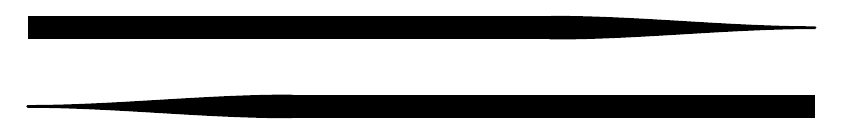
\begin{tikzpicture}
\pen (0,0);
\tikzset{heavy line width=3mm}
\calligraphy[heavy, taper=end] (0,0) -- +(10,0);
\calligraphy[heavy, taper=start] (0,-1) -- +(10,0);
\end{tikzpicture}



\begin{tikzpicture}
\pen (-135:.25) -- (45:.25);
\draw[line width=.5cm] (0,0) .. controls +(45:1) and +(-135:1) .. ++(3,0);
\calligraphy (0,-1) .. controls +(45:1) and +(-135:1) .. ++(3,0);
\end{tikzpicture}

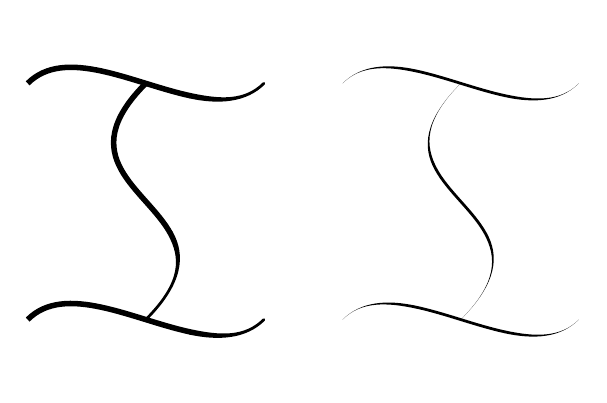
\begin{tikzpicture}[line width=2pt]
\pen (0,0);
\calligraphy[heavy,taper=end] (0,0) .. controls +(45:1) and +(-135:1) .. +(3,0) ++(1.5,0) .. controls +(-135:2) and +(45:2) .. +(0,-3)  (0,-3) .. controls +(45:1) and +(-135:1) .. +(3,0);
\calligraphy[light] (4,0) .. controls +(45:1) and +(-135:1) .. +(3,0) ++(1.5,0) .. controls +(-135:2) and +(45:2) .. +(0,-3)  (4,-3) .. controls +(45:1) and +(-135:1) .. +(3,0);
\end{tikzpicture}


\begin{tikzpicture}[line width=1pt]
\pen (-135:.125) -- (0,0) (45:.125);
\calligraphy (0,0) .. controls +(45:1) and +(-135:1) .. +(3,0) ++(1.5,0) .. controls +(-135:2) and +(45:2) .. +(0,-3)  (0,-3) .. controls +(45:1) and +(-135:1) .. +(3,0);
\end{tikzpicture}


\begin{tikzpicture}[thick]
%\pen (0,0);
\coordinate (a) at (0,.5);
\coordinate (b) at (.5,0);
\coordinate (c) at (0,-.5);
\coordinate (d) at (-.5,0);
\draw (d) to[bend left] (c) to[out=150,in=210] (c);
\end{tikzpicture}

\end{document}

% Local Variables:
% tex-output-type: "pdf18"
% End: